\section{Learning to adapt to opponents}
\label{sec:part3}

In the previous chapter we tried to create an algorithm to develop the default strategy for the APC. \\

The goal of this chapter is to further develop the strategy of APC to also adapt to the strategies of the opponents. This chapter will be mainly theoretical since it is based on the strategy of the previous chapter, which did not work.
%it did work! like awesome boss but without fold :(

\vspace{4mm}
\begin{statementBox2}{Problem statement 3}
How can we further develop the APC's strategy to be able to adapt to the playing style of the opponent?
\end{statementBox2}
\vspace{4mm} 

In poker there is no such thing as a single strategy that is better than any other strategy. Every strategy has weaknesses and therefore the optimal strategy is one that takes advantage of the weaknesses of the strategies of the opponents. In order to take advantage of the opponents strategy, one must first understand their strategy. In poker understanding the opponents is one of the most important key elements of the game. 

Once one understands the strategy of the opponent one has to adapt oneself's strategy.

Since poker is a game of deception the opponents may change their strategy during the game. In this case the player needs to find out about this and adapt the strategy once again. 

\subsection{Design}
Because the work of this strategy is based on the ANN from chapter \ref{sec:part2}, the focus of this chapter is on the theory rather than implementation and testing. The reason is, that the ANN from chapter \ref{sec:part2} did not end up working properly, and therefore it would not be possible to tell if the solution did not work, due to the original ANN or due to the improvements created in this chapter. 

Instead of implementing the improvements, we just suggest how we could have implemented them.\\

There is two commonly used approaches to develop a strategy that adapts to the strategy of the opponents.

The traditional approach is to use statistics to learn about the opponents. Such an approach uses probabilities based on the players actions to determine the strength of the players hand. Such probabilities may include but are not limited to, the percentage of hand the player folds during each game state, the percentage of times the player bluffs on the river, and the strength of the hand the player has when calling aggression. This is useful against a player who use the same strategy throughout the whole game and who's actions are deterministic.

The other approach is using player modelling, see section \ref{asd} and artificial neural networks (ANN), see section \ref{a}. This approach has gained increasing popularity through the recent years. In this approach the ANN is responsible of learning the strategy of the player. This approach is good for learning the strategy of a player who performs non-deterministic actions. It can also adapt in case the player changes strategy.\\

We choose to us the second approach and create a player model and an ANN. We find it more interesting to use player modelling and ANN's as this approach seems to have a lot of potential within the field of artificial intelligence in poker.

Aaron Davidson is a master of science from the University of Alberta. In his thesis about opponent modelling in poker \cite{opp-mod}, he uses ANN's in combination with player modelling in order to develop the poker computer Poki. An ANN was designed to predict the action of an opponent. The ANN uses a total of 17 player specific inputs. Using this design, Poki was able to win against most online poker players and computers but was far from world class.

G. Nicolai and R. Hilderman also made use of ANN's and player modelling in their thesis \cite{poker-agents}. They use a single ANN to determine the action of the computer. The model each player using overall aggressiveness and recent aggressiveness and give it as an input to the ANN. Although their computer agent was no way as advanced as Poki, it still showed potential.

Using ANN's in combination with player modelling looks like variable approach. In the rest of this chapter, we will discuss this approach and suggest a potential way of implementing it. We will start by introducing the concept of player modelling. We then design a player model suitable for the APC and finally design the ANN.

\subsubsection{Player modelling}
\label{sec:pm}
Player modelling is a loosely defined concept and may vary from one context to another. The concept of player modelling is to make a computational model of a player. This model includes game related attributes, such as play style and preferences, as well as non-game related attributes, such as cultural background, gender, and personality. All decisions of the player are ultimately made on the basis of these attributes. 

Player modelling is used to describe or predict the players decisions, reasoning and reactions. In the field of artificial intelligences the human player is the most used model for developing computer players. Understanding the reason behind every choice of a player will not only bring a better understanding of the player but also a better understanding of the game and its mechanics.

Since the player model can easily become extremely extensive one has to determine which attributes are relevant.

\subsubsection{Design of the player model}
It is crucial to figure out which attributes are relevant to the specific player model. When trying to model a player there is almost no limit to what could be included. Attributes such as state of mind, energy, and distractions affect the decision of every human player.  

Below we have listed the attributes that we find most relevant for poker.

\begin{description}
\item[Aggressiveness] How often does the player tend to bet or raise.
\item[Tightness] How strictly does the player's actions reflect the strength of the player's hand. For instance, a tight player will play aggressive when having a strong hand and defensive or fold when having a weak hand. A loose player may bluff (play aggressive while having a weak hand) and slow play (play defensive while having a strong hand) a lot.
\item[Riskiness] How easy is it to push the player to fold. Risky players tend to fold less often while under pressure from the opponents and are therefore harder to bluff.
\item[Body language] Most human players unconsciously show emotions through their body language. The professional poker players can often tell a lot about an opponent's hole cards solely by looking at the opponent's body language.
\item[Time of decision making] The time a player use for each decision can show the confidence of the players choice. A fast decisions indicates an easy decision. 
\end{description}

Since our APC is targeted towards computer players as well as human players, it makes no sense to use attributes such as body language and the time of decision making to model the opponents. Those attributes only affect human players. Instead we will model the opponents using the attributes aggressiveness, tightness, and riskiness.

Aggressiveness can be found by simply looking at the actions of the opponent. 

Tightness is a bit more complicated as we need to know the hole cards of the player. Therefore we can only track the tightness of rounds where the player makes it to the showdown.

Riskiness is also easy to measure. Riskiness shows how likely the player is to call while under pressure from opponents. We can determine the riskiness of the player by tracking the number of times the player folds contra the number of times the player calls or raises.

The APC needs to be able to recognise if a player changes strategy during the game. To accomplish this we split each attribute into the two attributes: overall and recent. Overall, covers every round throughout the game. Recent, only covers the last ten rounds.

The reason we choose  ten games, in our definition of recent, is because a player might get lucky and get several strong hole cards in a row. This may cause the player to play more aggressive than usual even though the player still uses the same strategy - resulting in a miss read by the player model. We found that ten games is enough to avoid miss-reads and also allows to track actual changes in the players strategy.

Aggressiveness is also split into one additional attribute called current aggressiveness, which is the players aggressiveness in previous game states of the current round.

We end up using the following attributes for our player model:
\begin{itemize}
\item Overall aggressiveness
\item Recent aggressiveness
\item Current aggressiveness
\item Overall tightness
\item Recent tightness
\item Overall riskiness
\item Recent riskiness
\end{itemize}

In the rest of this section we will describe one way we could have implemented the player model. Note that the player model has not been implemented but this is only a description of how we would have done it.

The aggressiveness of a round $n$ can be found as:

\[Agg,n = \frac{A_{bet},n + A_{raise},n}{A_{total},n}\]

$A_{agg},n$ is the player's number of bets $A_{bet},n$ and raises $A_{raise},n$ in round $n$ and  $A_{total},n$ is the player's total number of actions in round $n$. 

Overall aggressiveness can be found as the average aggressiveness of all rounds, recent aggressiveness would be found as the average aggressiveness of the last ten rounds and finally the current aggressiveness would be found as the average aggressiveness of the previous game states of the current round.\\

The tightness of the player can be found by backtracking the actions of the player after the round is finished. This is of course only possible for rounds that makes it to the showdown, since we otherwise do not know the hole cards of the player.

In order to determine if a player either bluffs or slow plays, we would have to establish some boundaries based on the hand strength. 

We took a sample of 100 defensive actions and 100 aggressive actions, and plotted the data in figure \ref{fig:dist-act}. The boundary for bluffing (red line) shows that the players tends to play defensive below this line. Likewise the boundary for slow play (blue line) shows that the players tends to play aggressive above this line.

\begin{figure}[H]
  \center
    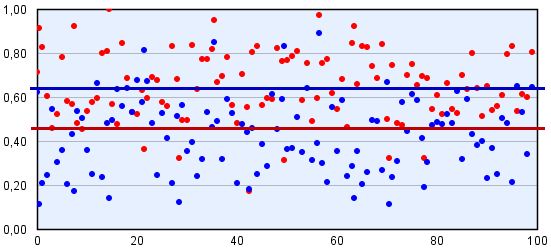
\includegraphics[scale=0.775]{images/modeling/action-dist.png}
  \caption{Distribution of actions in regards to the hand strength. Red dots indicates aggressive actions and blue dots defensive actions. The red line indicates the boundary for slow play and the blue line the boundary for bluffing. \label{fig:dist-act}}
\end{figure}

We define slow playing as playing defensive with a hand strength of more than 0,63.

We define bluffing as playing aggressive with a hand strength of less than 0,46.

We can then find the tightness of a round $n$ using the formula:

\[Ti,n = 1 - \frac{A_{bluff},n + A_{slow},n}{A_{total},n}\]

Here $A_{bluff},n$ is the number of times the player has bluffed in round $n$, $A_{slow},n$ is the number of times the player has slow played in round $n$ and $A_{total},n$ is the total number of actions in round $n$.

We can then find the overall- and recent tightness the same way as with the aggressiveness. Although we can only track the past ten rounds where the player made it to showdown.\\

Finally we can find the riskiness of a round $n$ as the number of times the player calls or raise in regards to the number of times it costs the player to continue:

\[Ri,n = \frac{A_{call},n + A_{raise},n}{A_{call},n + A_{raise},n + A_{fold},n}\]

Here we have the number of times the player calls $A_{call},n$, raises $A_{raise},n$ and folds $A_{fold},n$, all in round $n$.

\subsection{Combining the ANN and player model}
The ANN for the adaptive strategy would be based on the ANN design from section \ref{sec:design2}, see figure \ref{fig:nn2}. 

\def\layersep{2.5cm}

\begin{figure}[H]
\center
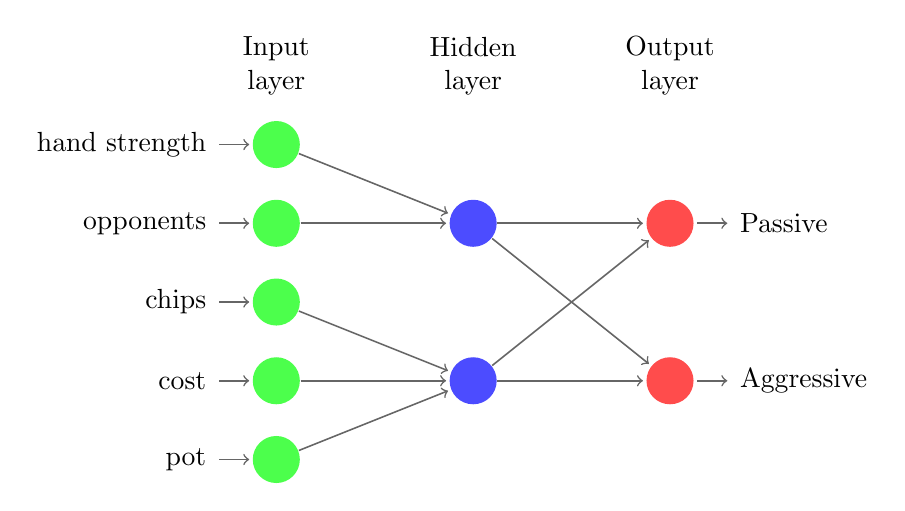
\begin{tikzpicture}[shorten >=1pt,->,line width=0.2mm,draw=black!60, node distance=\layersep]
    \tikzstyle{every pin edge}=[<-,shorten <=1pt]
    \tikzstyle{neuron}=[circle,fill=black!25,minimum size=17pt,inner sep=0pt]
    \tikzstyle{input neuron}=[neuron, fill=green!70];
    \tikzstyle{output neuron}=[neuron, fill=red!70];
    \tikzstyle{hidden neuron}=[neuron, fill=blue!70];
    \tikzstyle{annot} = [text width=4em, text centered]

    % Draw the input layer nodes
    %\foreach \name / \y in {1,...,4}
    % This is the same as writing \foreach \name / \y in {1/1,2/2,3/3,4/4}
    \node[input neuron, pin=left:hand strength] (I-1) at (0,-1) {};
    \node[input neuron, pin=left:opponents] (I-2) at (0,-2) {};
    \node[input neuron, pin=left:chips] (I-3) at (0,-3) {};
    \node[input neuron, pin=left:cost] (I-4) at (0,-4) {};
    \node[input neuron, pin=left:pot] (I-5) at (0,-5) {};

    % Draw the hidden layer nodes
    \node[hidden neuron] (H-1) at (\layersep,-2) {};
    \node[hidden neuron] (H-2) at (\layersep,-4) {};

    % Draw the output layer node
    \node[output neuron,pin={[pin edge={->}]right:Passive}] (O-1) at (2*\layersep,-2) {};
    \node[output neuron,pin={[pin edge={->}]right:Aggressive}] (O-2) at (2*\layersep,-4) {};

    % Connect every node in the input layer with every node in the
    % hidden layer.
    \path (I-1) edge (H-1);
    \path (I-2) edge (H-1);
    \path (I-3) edge (H-2);
    \path (I-4) edge (H-2);
    \path (I-5) edge (H-2);
    
    % Connect every node in the hidden layer with the output layer
    \path (H-1) edge (O-1);
    \path (H-1) edge (O-2);
    \path (H-2) edge (O-1);
    \path (H-2) edge (O-2);

    % Annotate the layers
    \node[annot,above of=I-1, node distance=1cm] (il) {Input layer};
    \node[annot,right of=il] (hl) {Hidden layer};
    \node[annot,right of=hl] {Output layer};
\end{tikzpicture}
\caption{Second ANN design. \label{fig:nn2}}
\end{figure}

We choose to use the approach by G. Nicolai and R. Hilderman and construct a single ANN that takes the attributes of the players as inputs. The target is to learn the ANN what to do, based on the inputs about the game and attributes of the opponents.

The inputs for the ANN can be seen in table \ref{ann-design}. The attributes of the players are the attributes found in the previous section. In case there is less than nine opponents all attributes of a non-existing player is set to zero. Since the input function finds the net input as the sum of all the weighted inputs all inputs that are zero will not affect the ANN.

\begin{table}[H]
\center
\begin{tabular}{ | l | l | }
\hline
input & feature \\
\hline
1 & hand strength of APC\\
2 & number of opponents\\
3 & chips of the APC\\
4 & cost of the APC\\
5 & pot\\
6 to 12 & attributes of opponent 1\\
13 to 19 & attributes of opponent 2\\
20 to 26 & attributes of opponent 3\\
27 to 33 & attributes of opponent 4\\
34 to 40 & attributes of opponent 5\\
41 to 47 & attributes of opponent 6\\
48 to 54 & attributes of opponent 7\\
55 to 61 & attributes of opponent 8\\
62 to 68 & attributes of opponent 9\\
\hline
\end{tabular}
\caption{Inputs for the ANN design \label{tab:ann-design}}
\end{table} 

\subsection{Discussion}
In this chapter we discuss how we could have improved the strategy of the APC to also take the opponent's play style into account. 

We choose to use player modelling to model the opponents using seven attributes. 


\subsection{Conclusion}
In this chapter we discuss and suggest a solution to problem statement 3.

\vspace{4mm}
\begin{statementBox2}{Problem statement 3}
How can we further develop the APC's strategy to be able to adapt to the playing style of the opponent?
\end{statementBox2}
\vspace{4mm} 

One can either use a statistically approach or an approach using player modelling. We choose to use the approach using player modelling. 

For our approach we use player modelling to find relevant attributes to define an opponent. These attributes will then be given as inputs to an ANN which then determines the action of the APC. 

We find the following relevant attributes for the player model.

\begin{description}
\item[Aggressiveness] refers to how often the player bets or raises.
\item[Tightness] refers to how strictly the player's actions reflect the strength of the player's hand.
\item[Riskiness] refers to how often the player pays to continue instead of folding.
\end{description}

To make it possible for the APC to detect changes in the strategy of an opponent we split each attribute into an overall attribute and recent attribute. The overall attribute is the average of every round though the entire game whereas the recent attribute is the average of the last ten rounds. A change in strategy will affect the recent attribute and cause the APC to detect the change.

Aggressiveness has been split into one additional attribute called current aggressiveness which is the aggressiveness of the previous game states of the current round.

We end up with a total of 7 attributes:
\begin{itemize}
\item Overall aggressiveness
\item Recent aggressiveness
\item Current aggressiveness
\item Overall tightness
\item Recent tightness
\item Overall riskiness
\item Recent riskiness
\end{itemize}

We suggest the following way of finding the attributes.

The aggressiveness of a round can be found as the number of times the player bets or raise divided by the total number of actions of the player for that round.

The aggressiveness of a round can be found as the number of times the player bluffs or slow plays divided by the total number of actions of the player for that round.

The riskiness of a round can be found as the number of times he calls or raises divided by the total number of times the player has to pay in order to continue.\\

We then designed a new ANN that took the attributes for each a player as additionally inputs. The 68 inputs for the ANN can be seen in table \ref{tab:ann-design-con}. 

\begin{table}
\center
\begin{tabular}{ | l | l | }
\hline
input & feature \\
\hline
1 & hand strength of APC\\
2 & number of opponents\\
3 & chips of the APC\\
4 & cost of the APC\\
5 & pot\\
6 to 12 & attributes of opponent 1\\
13 to 19 & attributes of opponent 2\\
20 to 26 & attributes of opponent 3\\
27 to 33 & attributes of opponent 4\\
34 to 40 & attributes of opponent 5\\
41 to 47 & attributes of opponent 6\\
48 to 54 & attributes of opponent 7\\
55 to 61 & attributes of opponent 8\\
62 to 68 & attributes of opponent 9\\
\hline
\end{tabular}
\caption{Inputs for the ANN design \label{tab:ann-design-con}}
\end{table}
